\chapter{Analysis}\label{sec:analysis}
One purpose of this section is to abstract and deduce the essential characteristics of any interaction.
These characteristics are relevant for a formalized language of \cmvs{}.
To accomplish this goal, we take the approach of deducing the characteristics by example.
We analyze each data visualization example in terms of the expected data structure and dependent and independent visual variables~\cite{Bertin2010}.
We suggest interactions for each visualization as well as interactions that run on multiple views.
Those interactions will be classified according to \textcite{Yi2007} and the relevant subject of the interaction is specified.

The second outcome of this section is a set of requirements which can be used to evaluate a framework of \cmvs{}.


\section{Single Visualization Interactions}\label{sec:analysis:examples:single}

The data visualization catalogue by Severino Ribecca list many of the most used data visualizations\cite{VisualizationCatalogue2017}.
Let's pick some of those and derive a number of possible interactions.

%\begin{tabular}{l l l l}
    %Comparisons & Proportions & Relationships & Hierarchy \\
    %Concepts & Location & Part-to-a-whole & Distribution \\
    %How things work & Processes \& methods & Movement or flow & Patterns \\
    %Range & Data over time & Analysing text & Reference tool \\
%\end{tabular}


\textbf{Line diagrams}
\begin{figure}
  \begin{center}
    \subfloat[Line diagram]{{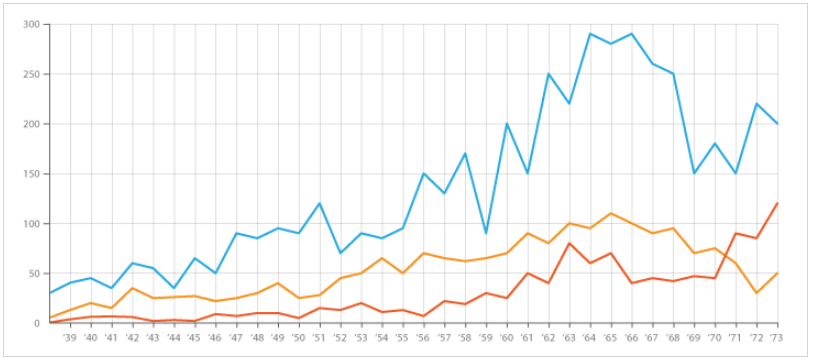
\includegraphics[width=0.4\textwidth]{images/chartTypes/line-diagram.png} }}%
    \qquad
  \end{center}
  \caption{Line charts are used to display trends}\label{fig:concept:chart-types:line-diagrams}
\end{figure}

Line diagrams are multiple sets of data, displayed along the x-axis.
They are used to display quantitative value over a continuous interval or time span.
It is possible to highlight an entire series of data or just a feature within that series.

\conceptTable{Tabular data, many data sets as series.}{Position, orientation, texture.}{Color, shape, size.}

\begin{figure}
    \begin{center}
        \caption{Interactions for line charts}%
        \label{fig:concept:chart-types:line-diagrams:interactions}
        {\small
            \begin{tabulary}{\textwidth}{ll}
                \bf Select & Highlight a data point (id of data point) \\
                \bf Select & Highlight a data series (id of data series) \\
                \bf Encode & Change colours of data series (data series \rightarrow\ colour) \\
                \bf Filter & Restrict interval on x-axis (filter function of data attribute) \\
                \bf Filter & Hide a data series (id of data series) \\
            \end{tabulary}
        }
    \end{center}
\end{figure}



\textbf{Bar charts and multiset bar charts}

\begin{figure}
  \begin{center}
    \subfloat[Bar chart]{{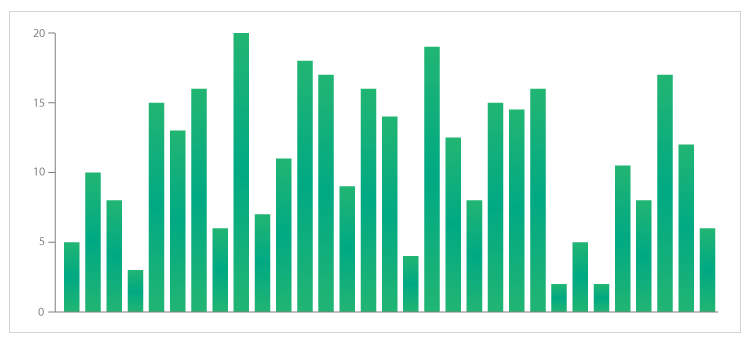
\includegraphics[width=0.4\textwidth]{images/chartTypes/bar-chart.png} }}%
    \qquad
    \subfloat[Multiset bar chart]{{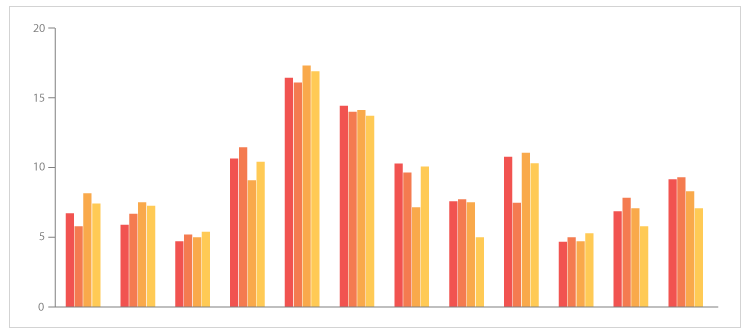
\includegraphics[width=0.4\textwidth]{images/chartTypes/multiset-bar-chart.png} }}%
  \end{center}
  \caption{A multiset bar charts is a variation of a bar chart}\label{fig:concept:chart-types:bar-charts}
\end{figure}

Bar charts and multiset bar charts show one or many attributes per feature along an axis.
They have in common that they encode the data attribute into the height of the eponymous bars.
Colors might be used to better distinuish between the different data attributes.
Features can be arbitrarily ordered along the axis, although multiset bar charts group features along a series of categories.

Therefore, bar charts need to be initialized with the set of features and their values as well as the groups of features for the multiset bar chart.
The supplied colours would colour each feature in a group in turn.
The set of possible ineractions include the highlighting of features, the reordering of features and a change in encoding of colour values.

\conceptTable{Tabular data, many data sets as series}{Size, orientation.}{Position, colour, shape, texture.}

\begin{figure}
    \begin{center}
        \caption{Interactions for bar charts}\label{fig:concept:chart-types:bar-charts:interactions}
        {\small
            \begin{tabulary}{\textwidth}{ll}
                \bf Select & Highlight a bar (id of data point) \\
                \bf Encode & Change colours of data series (colours \rightarrow{} data series) \\
                \bf Reconfigure & Sort by attribute (data attribute) \\
                \bf Reconfigure & Drag bars to reorder data series (ordered list of ids of data points) \\
                \bf Filter & Hide a data series (id of data series) \\
            \end{tabulary}
        }
    \end{center}
\end{figure}


\begin{figure}
  \centering
    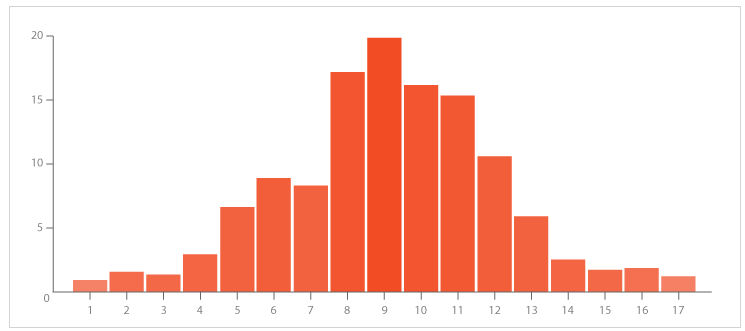
\includegraphics[width=0.4\textwidth]{images/chartTypes/histogram.png}%
    \label{fig:concept:chart-types:histograms}
    \caption{A histogram is a bar chart over a continuous interval}%
\end{figure}

Histograms visualise the distribution of data over a continuous interval or certain time period.
A special type is the population pyramid, which is a pair of back-to-back histograms, one for each sex.
The difference of histograms to bar charts lies in the type of data itself, not the representation.
Therefore these charts need to be initialized with the same data and the same interactions can be applied.

\conceptTable{Tabular data, many data sets as series}{Size, orientation, position.}{Color, shape, texture.}

\textbf{Bubble charts and scatter plots}

\begin{figure}
  \centering
    \subfloat[Bubble chart]{{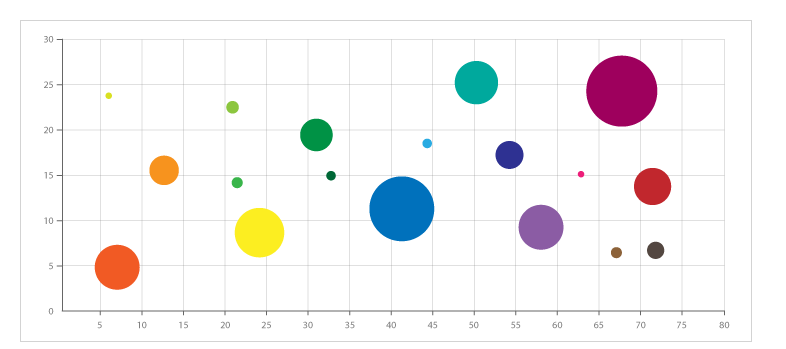
\includegraphics[width=0.4\textwidth]{images/chartTypes/bubble-chart.png} }}%
    \qquad
    \subfloat[Scatter plot]{{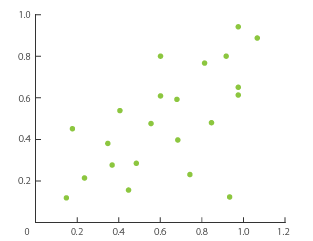
\includegraphics[width=0.4\textwidth]{images/chartTypes/scatter-plot.png} }}%
    \caption{Bubble charts and scatter plots are similar regarding interactions}%
    \label{fig:concept:chart-types:bubble-chart}
\end{figure}

Bubble charts are popular choices to display a distribution of features.
The chart is initialized with coordinates for each feature, a colour and a size in case of a bubble charts.
Possible interactions include the highlighting of features, a different colour encoding, a reconfiguration to map another attribute to size.
Bubble charts may show only a window of the available data and allow to zoom in, zoom out or move the window along the axes.

\conceptTable{Tabular data, single data set with x- and y-coordinates}{Size, position.}{Color, shape, texture, orientation.}

\begin{figure}
    \begin{center}
        \caption{Interactions for bubble charts}%
        \label{fig:concept:chart-types:bubble-chart:interactions}
        {\small
            \begin{tabulary}{\textwidth}{ll}
                \bf Select & Highlight a bubble (id of data point) \\
                \bf Explore & Zoom in, zoom out (width and height of window) \\
                \bf Explore & Move viewport position (x- and y-coordinates of viewport) \\
                \bf Encode & Change mapping of colour to category (data series \rightarrow\ colour) \\
                \bf Encode & Change colour function (function value \rightarrow\ colour) \\
                \bf Encode & Change data attribute to colour (data attribute) \\
                \bf Encode & Change data attribute to size \\
                \bf Reconfigure & Sort by attribute (data attribute) \\
                \bf Reconfigure & Drag bars to reorder data series (ordered list of ids of data points) \\
                \bf Filter & Hide a data series (id of data series) \\
            \end{tabulary}
        }
    \end{center}
\end{figure}

\textbf{Stacked bar charts}

\begin{figure}
  \centering
    \subfloat[Stacked bar chart]{{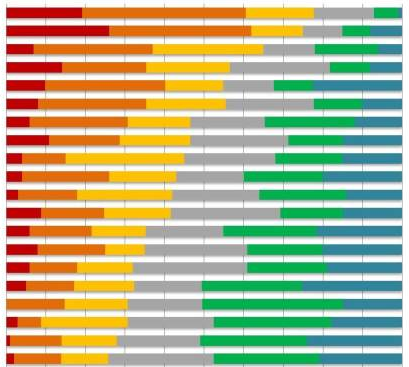
\includegraphics[width=0.3\textwidth]{images/chartTypes/stacked-bar-without-baseline.png} }}%
    \qquad
    \subfloat[Stacked bar chart with baseline]{{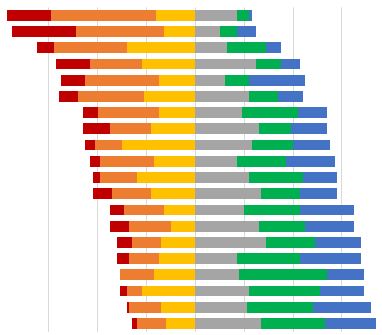
\includegraphics[width=0.3\textwidth]{images/chartTypes/stacked-bar-with-baseline.png} }}%
    \caption{Stacked bar charts can be ordered along a baseline or stretch to 100\% width to show the percentage-of-the-whole of each group}%
    \label{fig:concept:chart-types:stacked-bar-chart}
\end{figure}
\begin{figure}
  \centering
    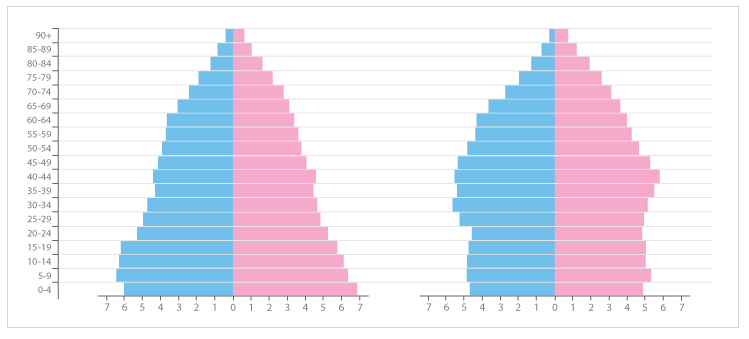
\includegraphics[width=0.4\textwidth]{images/chartTypes/population-pyramid.png}%
    \label{fig:concept:chart-types:population-pyramid}
    \caption{A population pyramid can be modeled as a stacked bar chart}%
\end{figure}

Unlike a multi-set bar graph which displays their bars side-by-side, stacked bar graphs segment their bars of multiple datasets on top of each other.
A baseline, as shown in figure~\ref{fig:concept:chart-types:stacked-bar-chart} might be modeled as two back-to-back multi-set bar graphs. A reordering would e.g.\ move one data set from the left side to the right side.
Possible interactions include the highlighting of a feature, a change of color mapping, reordering of the baseline.

\begin{figure}
    \begin{center}
        \caption{Interactions for stacked bar charts}%
        \label{fig:concept:chart-types:stacked-bar-chart:interactions}
        {\small
            \begin{tabulary}{\textwidth}{ll}
                \bf Select & Highlight a bar (id of data point) \\
                \bf Encode & Change mapping of category to colour (data series \rightarrow\ colour) \\
                \bf Reconfigure & Sort by attribute (data attribute) \\
                \bf Reconfigure & Reorder Y axis (ordered list of ids of data points) \\
                \bf Reconfigure & Sort stacking order by attribute (data attribute) \\
                \bf Reconfigure & Specify the stacking order data series (ordered list of ids of data series) \\
                \bf Reconfigure & Specify a negative data series (list of ids of data series) \\
                \bf Filter & Hide a data series (id of data series) \\
            \end{tabulary}
        }
    \end{center}
\end{figure}

\conceptTable{Tabular data, multiple date sets as series}{Size, shape, orientation.}{Color, position, texture.}

\textbf{Hierarchical visualizations}

\begin{figure}
  \centering
    \subfloat[Tree map]{{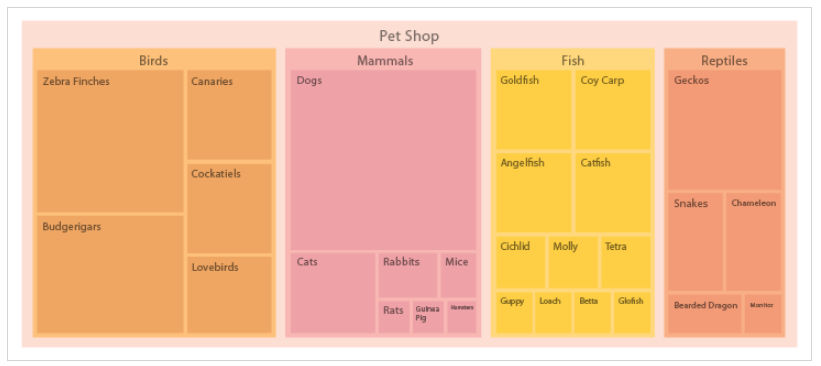
\includegraphics[width=0.4\textwidth]{images/chartTypes/treemap.png} }}%
    \qquad
    \subfloat[Sunburst diagram]{{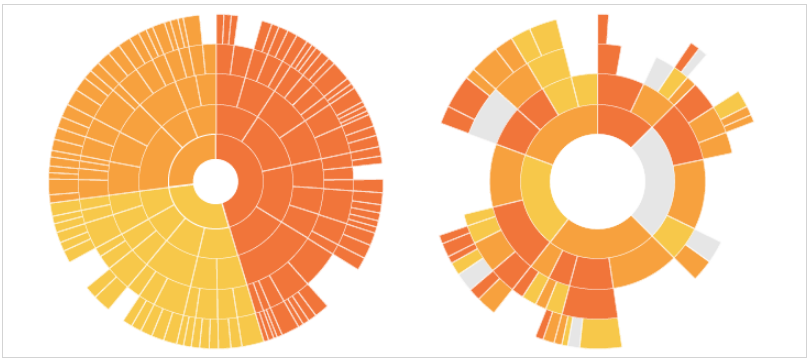
\includegraphics[width=0.4\textwidth]{images/chartTypes/sunburst.png} }}%
    \caption{Tree maps and sunburst diagrams are ideal to show hierarchies}%
    \label{fig:concept:chart-types:hierarchies}
\end{figure}

Treemaps are great to show hierarchical data without ever exceeding the availabe screen.
Each feature is a assigned a rectangle according to a layouting algorithm.
Unlike a tree map a hiearchical ring diagram or sunburst diagram shows each level of the tree as a series of rings.

Therefore, both tree map and ring diagram need the feature set as a tree, with each node having a data attribute for layouting. Every node may be assigned a color.
As we are describing hierarchies, the maximal depth of tree may be increased or decreased.
Again, interactions could include a highlighting of features and a change of color encoding.
Both visualizations may show only a subtree.
E.g.\ a click on a box in the treemap opens another treemap focused on the subtree.
Similarly a click on a slice of the ring would surround the most external ring with the children of the feature.

\conceptTable{Tree, each feature has a value for layouting.}{Position, Size, shape, orientation.}{Color, texture.}

\begin{figure}
    \begin{center}
        \caption{Interactions for hierarchical visualizations}%
        \label{fig:concept:chart-types:hierarchies:interactions}
        {\small
            \begin{tabulary}{\textwidth}{ll}
                \bf Select & Highlight a feature (id of data point) \\
                \bf Explore & Use another node as root of the visible tree (id of data point) \\
                \bf Encode & Change mapping of category to colour (data series \rightarrow\ colour) \\
                \bf Reconfigure & Change data attribute used for layouting (data attribute) \\
                \bf Reconfigure & Sort by attribute (data attribute) \\
                \bf Reconfigure & Specify order (ordered list of ids of data points) \\
                \bf Abstract/Elaborate & Specify maximum depth of visible tree (number of levels) \\
            \end{tabulary}
        }
    \end{center}
\end{figure}

\textbf{Geographical Data}

\begin{figure}
  \centering
    \subfloat[Choropleth map]{{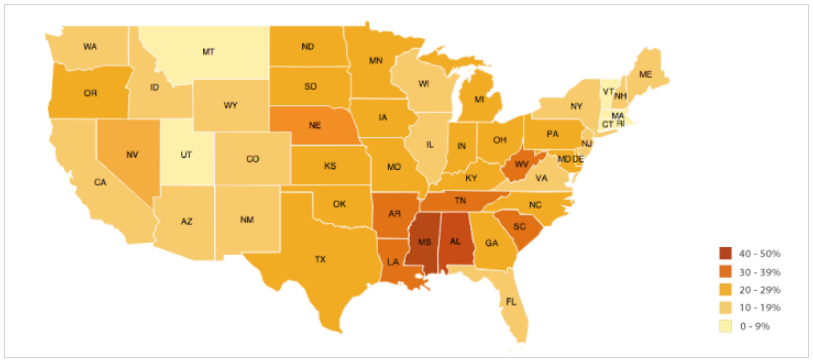
\includegraphics[width=0.4\textwidth]{images/chartTypes/choropleth-map.png} }}%
    \qquad
    \subfloat[Flow map]{{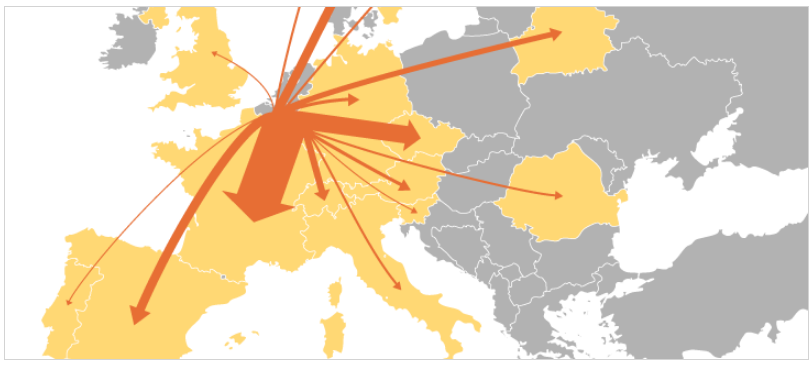
\includegraphics[width=0.4\textwidth]{images/chartTypes/flow-map.png} }}%
    \caption{Choropleth maps focus on a density while flow maps show a migration of data}%
    \label{fig:analysis:chart-types:geographical}
\end{figure}

Choropleth maps and flow maps are specialized diagrams focused on geographical data.
Size, position and shape of a feature is defined by the geometry data of a feature.
In choropleth maps the color of each feature is based on a data attribute.
Flow maps may display connections between features, a data value defining the size of each arrow.

\conceptTable{Graph data with edges, each feature has geometry data.}{Position, Size, shape, orientation.}{Color, texture.}

\begin{figure}
    \begin{center}
        \caption{Interactions for geographical visualizations}%
        \label{fig:concept:chart-types:geographical:interactions}
        {\small
            \begin{tabulary}{\textwidth}{ll}
                \bf Select & Highlight a feature (id of data point) \\
                \bf Explore & Move viewport (latitude and longitude of viewport)\\
                \bf Explore & Zoom in, zoom out (zoom factor) \\
                \bf Encode & Change shape of marker (data id \rightarrow\ shape) \\
                \bf Encode & Change mapping of category to colour (data series \rightarrow\ colour) \\
                \bf Encode & Change colour function (value \rightarrow\ colour) \\
                \bf Encode & Change data attribute used for colour (data attribute) \\
                \bf Connect & Show relations of a feature (id of data point)  \\
                \bf Abstract/Elaborate & Change granularity of displayed regions (number of levels) \\
            \end{tabulary}
        }
    \end{center}
\end{figure}

\textbf{Activity diagrams}
\begin{figure}
  \centering
    \subfloat[Calendar]{{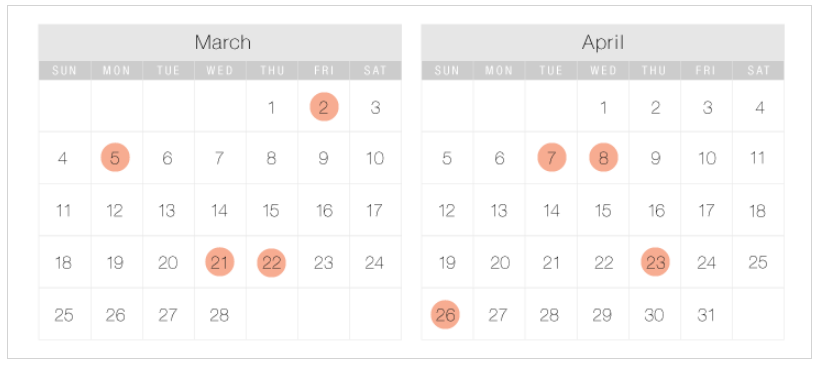
\includegraphics[width=0.4\textwidth]{images/chartTypes/calendar.png} }}%
    \qquad
    \subfloat[Gantt chart]{{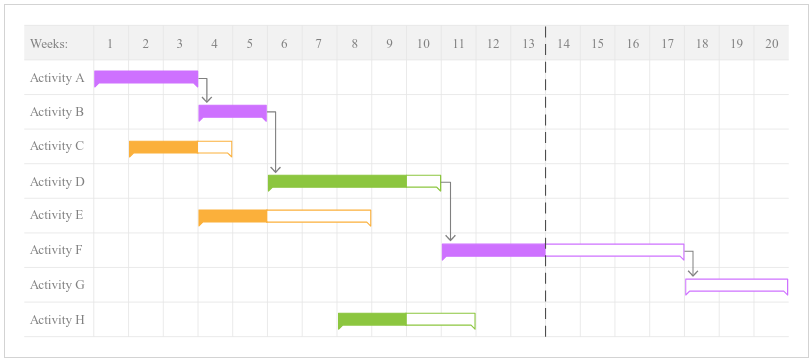
\includegraphics[width=0.4\textwidth]{images/chartTypes/gantt-chart.png} }}%
    \caption{Similar to a calendar, a gantt chart shows activities and the progress along a time line}%
    \label{fig:concept:chart-types:temporal}
\end{figure}

In activity diagrams, each feature is represented as a rectangle, with the duration of the activity mapped to size and position.
Calendars and gantt charts could not only read the data from the data source, but also add new features to the data set or update metadata of a feature, e.g.\ the progress of the activity.

\conceptTable{Temporal data, each feature has a time interval.}{Position, Size, orientation.}{Color, shape, texture.}

\begin{figure}
    \begin{center}
        \caption{Interactions for temporal visualizations}%
        \label{fig:concept:chart-types:temporal:interactions}
        {\small
            \begin{tabulary}{\textwidth}{ll}
                \bf Select & Highlight a feature (id of data point) \\
                \bf Explore & Show a different period of dates (start and end datetime)\\
                \bf Explore & Show a different time interval (start and end hour)\\
                \bf Encode & Change color of categories or activities (data series \rightarrow\ colour) \\
                \bf Encode & Change data attribute used for colour (data attribute) \\
                \bf Filter & Remove a calendar or a category (id of data series) \\
            \end{tabulary}
        }
    \end{center}
\end{figure}

\section{Multiple View Interactions}\label{sec:analysis:examples:multiple}

\textbf{Detail view}
\begin{figure}
  \centering
  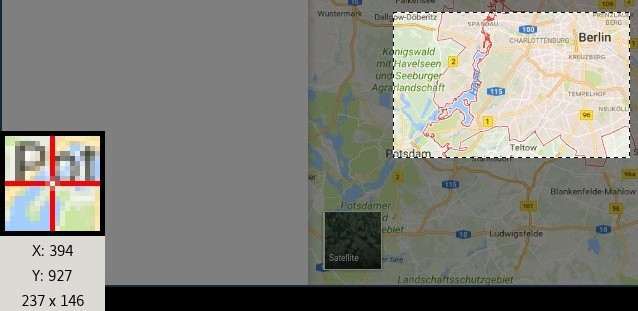
\includegraphics[width=0.4\textwidth]{images/chartTypes/multi/detail-view}
  \caption{The screenshot-tool ``shutter'' shows a magnified detail view of the area around the mouse cursor in the lower right corner of the screen}\label{fig:concept:chart-types:detail}
\end{figure}

\section{Requirements}
In this subsection, we list a set or requirements imposed on a \cmv{} framework.
These requirements can be used for further evaluation.
\textbf{Serialization} is the process of translating objects that can be stored or transmitted and reconstructed later.
In order to coordinate interactions among views, information needs to be passed from one view to another. 
A framework for \cmvs{} should therefore find a serialization format for interactions which has
\begin{enumerate*}[label=(\arabic*)]
  \item
    small payloads and
  \item 
    fast serialization and deserialization.
\end{enumerate*}

\textbf{Reversibility} in the context of a \cmv{} framework means if it is possible to undo the effect of an interaction.
Ideally, every interaction function should have a well-defined inverse.
For every interaction that is not reversible, the computational cost to replay the interactions from the original state up to the point of the interaction should be minimal.

\textbf{Data extensibility} indicates the ease of reloading and updating data on the fly.
This is especially important if an interaction requests additional data from an external service.
We consider good extensibility when
\begin{enumerate*}[label=(\arabic*)]
  \item
    additional data attributes can be added without lookup of corresponding items and
  \item
    no de-duplication steps are necessary when new items are added.
\end{enumerate*}

\textbf{Development costs} qualify how much time and effort is needed in order to develop new components for the \cmv{} framework.
We track these costs in working days and the number of changed lines of code.


\textbf{Maintainability} means in our case, how much other views are impacted by a change of an interaction in one view and how error-prone the framework is.
In general it is hard to measure maintainability.
For the \cmv{} framework we want to measure the
\begin{enumerate*}[label=(\arabic*)]
  \item
    lines of code and the
  \item
    cycliomatic complexity. We will try to find a means to measure
  \item
    cohesion and
  \item 
    coupling in the framework.
\end{enumerate*}
We assume that the amount of shared data between views is an indicator for high coupling.





\begin{bullshit}
\section{Free visual variables allow for interaction effects}

In order to communicate the interaction to the user, the effect of the visualization must be communicated back to the user by a visual change.
Data visualizations have \emph{dependent} and \emph{independent} visual variables, see~\ref{sec:related-work:visual-variables}.
Dependent variables are those that are tied to a data attribute.
These constrained visual attributes are unavailable while independent visual variables are therefore available to be used for a visual feedback of an interaction.

\section{List events as candidates for interaction triggers}

Interaction can be triggered by any input of a human-computer-interaction device, like the keyboard or the mouse.
Because users are in the habit of expecting certain interactions to be triggered from certain events, we also have constraints here.
E.g.\ the viewpoint in geographical maps is moved by mouse drag events and the zoom level is controlled by the mouse wheel.
So we should not use those already occupied events as triggers for our coordinated interactions.
Nevertheless, consistency in user interfaces is crucial for great user experience, because users can reuse the learned knowledge.
Therefore, we need to list all availabe events as candidates and connect them to our interactions in a preferrably consistent manner.

On the other hand, we might have special controls in visualizations, in order to change the encoding.
E.g.\ a \tmap{} shows a menu where the user can define how attributes are mapped to visual variables.
\end{bullshit}

